\problemname{Fire Hydrant}
\noindent
Firefighter Robert has been working as a firefighter for over 20 years and loves his job. 
After a long walk in the metropolis M (formerly known as Stockholm), Robert received a 
call on his phone from his hydrophobic chief, ordering him to come to the fire station 
right away. Robert has just arrived at the most south-west four-way intersection in 
metropolis M and decides to head straight to the fire station, but apparently, 
several fire hydrants in metropolis M have started leaking water and flooding the streets! 
Oh no! This is particularly serious because Robert's hydrophobic chief at the fire 
station is extremely strict about not having water near him, so showing up soaking 
wet to work after encountering several of the leaking fire hydrants will get Robert fired. 
Robert wants to work as a firefighter for at least 20 more years, so help Robert 
minimize how wet he gets!

Metropolis M consists of a grid with dimensions $W \times H$, where each four-way 
intersection is a square in the grid, and is reachable from the four adjacent 
intersections in each cardinal direction: north, east, south, and west. 
Robert has just arrived at the four-way intersection furthest southwest in the grid, 
at position $(1,1)$. Robert wants to reach the fire station furthest northeast in the grid, 
at position $(W,H)$. It takes exactly 1 minute to run from one four-way intersection to another 
adjacent intersection. It is guaranteed that the fire station is not located at $(1,1)$. 

Furthermore, there are $N$ four-way intersections with a leaking fire hydrant, 
which can be located in any square on the grid, including where Robert starts from $(1,1)$ and 
at the fire station $(W,H)$. Robert arrives at the square $(1,1)$ at minute 0, and each leaking 
fire hydrant has leaked one unit of water to the intersection the fire hydrant is located at. 
For each minute $t$ that passes, each leaking fire hydrant will leak an additional unit of water 
to all intersections within a certain distance from it. Specifically, all squares $(x,y)$ that 
satisfy the following inequality at minute $t$ will increase by one unit of water from the fire 
hydrant located at $(x_b,y_b)$:
$$
|x-x_b|+|y-y_b|\le t.
$$

Let's call the number of units of water at a particular square $v_t$ at minute $t$. 
When Robert arrives at a four-way intersection at minute $t$, Robert's clothes will get wet 
from all the water present at that intersection from leaking fire hydrants, which is $v_t$ units of water.

What is the minimum total number of water units that Robert needs to go through on his way to the fire station?


\begin{centering}
  \begin{figure}[h]
    \centering
  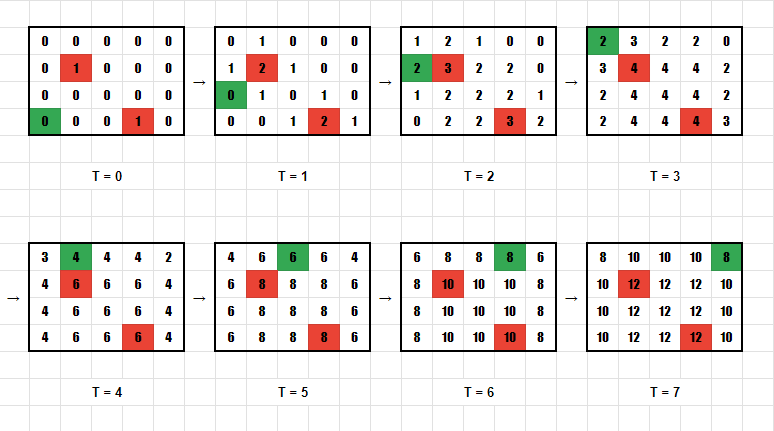
\includegraphics[width=1\textwidth]{brandpostSample1.png}
    \caption{Illustration of sample 1, where the green square is Roberts position and the
    red squares are the positions of the fire hydrants. The smallest total water units
    Bob can have when arriving at the station is $0+0+2+2+4+6+8+8=30$.}
    \label{fig:brandpost}
  \end{figure}
\end{centering}

\section*{Input}
The first line of the input contains three integers $W,H,N$ ($1 \le W,H \le 1000$, $1 \le N \le min(20000,W \cdot H)$), 
where $W$ and $H$ are the width and height of the grid and $N$ is the number of leaking fire hydrants.

The following $N$ rows each contain two integers $x_i$ and $y_i$ ($1 \le x_i \le W$, $1 \le y_i \le H$),
where $(x_i,y_i)$ is the position of the $i$:th leaking fire hydrant. It is guaranteed that no two
fire hydrants occupy the same cell.

\section*{Output}
Print an integer, the minimum number of water units Robert has to pass through on his way to the fire station.

\section*{Points}
Your solution will be tested on several test case groups.
To get the points for a group, it must pass all the test cases in the group.

\noindent
\begin{tabular}{| l | l | p{12cm} |}
  \hline
  \textbf{Group} & \textbf{Point value} & \textbf{Constraints} \\ \hline
  $1$    & $10$       & $W,H \le 10$, $N=1$ and the only fire hydrant is located at $(1,1)$. \\ \hline
  $2$    & $15$       & $W,H,N \le 50$ \\ \hline
  $3$    & $17$       & $W,H \le 100$, $N\le 200$\\ \hline
  $4$    & $27$       & $W,H \le 150$ \\ \hline
  $5$    & $31$       & No additional constraints. \\ \hline
\end{tabular}
